\part{Expérimentations}
Nous avons désormais un langage capable d'interroger tout type de données et nous avons aussi un intergiciel capable d'exécuter ces requêtes. Nous allons maintenant mettre en pratique ces idées. Tout d'abord, nous consacrons un chapitre à l'observation du réseau domestique. Puis, afin d'évaluer les performances de notre intergiciel, nous présentons une évaluation des performances dans un second chapitre.

\begin{savequote}[6cm]
<< What is this place

Filled with so many wonders?

Casting its spell

That I am now under >>

\qauthor{Fluttershy, So Many Wonders}
\end{savequote}

\chapter{DomVision : Application au réseau local domestique}
\chaptertoc
Nous avons présenté dans le chapitre d'introduction le contexte fil rouge sur lequel cette thèse s'appuie. Ce chapitre permet de mettre en pratique la solution d'observation. DomVision est l'instanciation d'Astronef-Asteroid sur le réseau local domestique. Ainsi, en quelques composants et en plusieurs requêtes, nous arrivons à mettre en œuvre un système d'observation.

Dans ce chapitre, nous présentons les différents points de mise en application qui nous permettent de valider notre contribution dans son ensemble. En premier lieu, dans la section~\ref{sec:valid:domvision:systeme}, nous présentons comment nous nous sommes adapté au système observé. Ensuite, en section~\ref{sec:valid:domvision:requetes}, nous détaillons les requêtes que nous avons pu déployer grâce à l'expressivité d'Astral. Cela couvre la mise à jour de la base de données comme les requêtes de l'utilisateur. Enfin, en section~\ref{sec:valid:domvision:architecture} nous démontrons la flexibilité de notre solution en introduisant un nouvel opérateur capable d'établir des préférences sur les observations.

\section{Adaptation au système observé}\label{sec:valid:domvision:systeme}
Dans cette section, nous analysons le système au sens où nous l'avons décrit jusqu'ici dans Astronef et Asteroid. Nous devons modéliser le système pour en extraire son schéma qui permet de représenter le catalogue dans la base d'Asteroid. Puis nous nous intéressons aux données temps-réel. En enfin, nous présentons les flux à notre disposition dans ce réseau.

\subsection{Le schéma du système}
Nous présentons ici la vision que nous avons du système que nous observons. Il est important de voir que cette vision ne doit pas être liée aux sources de données disponibles. Elle a pour but de refléter l'interprétation des experts souhaitant observer le système.

Pour chaque concept, il est nécessaire de pouvoir identifier les objets du système pour pouvoir leur associer nos observations. Ainsi, nous détaillons les attributs permettant de désigner un objet de façon unique. Toutefois, dans la pratique, les données collectées sont partielles et ces attributs peuvent être absents. Ces inconsistances peuvent être minimisées par l'utilisation d'heuristiques. Les conséquences de telles inconsistances seraient la création de plusieurs entrées dans le catalogue qui représentent le même objet du système.

Chaque concept est caractérisé par un ensemble de propriétés \textit{statiques}, relatives à sa description, et \textit{stables}, relatives à son état. Les données volatiles sont présentées dans la section suivante. Nous définissons ici trois concepts principaux : les équipements, les applications et les interfaces réseau.

\subsubsection{Équipements}
La notion d'équipement est une vision orientée utilisateur. En effet, un \textit{équipement} est un châssis physique. Les équipements virtuels ne sont pas représentés. Ce choix permet de représenter à l'utilisateur les appareils qu'il est capable de voir et de manipuler (débrancher par exemple). Quelques exemples : \textit{Livebox}, \textit{STB}\footnote{Set Top Box : Boitier connecté à une télévision pour fournir les services de partage de contenus, de télévisions, VOD...}, Ordinateurs, Tablettes, Disques durs réseaux.

\textbf{Identification} : un équipement \textit{peut} avoir un \textit{numéro de série} unique. L'utilisation des interfaces ou applications liées permet un moyen alternatif.

\subsubsection{Applications}
Nous désignons par \textit{application} un programme instancié sur un des équipements. À un \textit{équipement} est associé plusieurs \textit{applications}. Les \textit{applications} permettent d'effectuer des tâches sur leurs équipements respectifs. Une \textit{application} en exécution a un état. Dans cette expérimentation, nous ne considérons que \textit{actif} et \textit{inactif}. Plusieurs autres statuts pourraient être utilisés comme \textit{suspendu} ou \textit{gelé}. Notons que la détermination des statuts est généralement complexe, car le système fournit rarement des données précises à ce sujet puisque cela consiste en un autodiagnostic\footnote{L'utilisation d'inférences de haut niveau comme vu en section~\ref{sec:rw:supervision:contexte} peut devenir intéressante dans ces cas.}. Quelques exemples : Partage de contenu, Agent d'administration, Gestion d'impression. Une \textit{application} a un \textit{nom}, une \textit{description} textuelle et potentiellement un \textit{type}.

\textbf{Identification} : une application \textit{peut} fournir un \textit{nom} unique par l'utilisation d'un \textit{UUID}, par exemple. Alternativement, nous pouvons exploiter l'unicité de son \textit{type}. Par exemple, il n'existe qu'une application de passerelle internet sur le réseau domestique.

\subsubsection{Interfaces réseaux}
Les \textit{interfaces réseaux} sont moins sujets à interprétation que les deux concepts précédents. Une \textit{interface réseau} représente un point de connexion que possède un \textit{équipement} vers le réseau domestique. Nous supposons que cette interface est une interface \textit{MAC}\footnote{Permettant des interfaces \textit{IP} et \textit{Zigbee} potentiellement}. Elle possède un \textit{nom} système unique pour l'équipement, un type (wifi, Ethernet), ainsi qu'une adresse \textit{MAC} considéré unique sur le réseau et d'autres adresses comme \textit{IPv4} ou \textit{v6}.

\textbf{Identification} : seule l'adresse \textit{MAC} garantit l'unicité. Si elle n'est pas renseignée, l'adresse \textit{IP} peut être utilisé comme moyen alternatif.

\subsubsection{Concepts supplémentaires possibles}
Ayant une modélisation des concepts principaux du réseau local domestique, nous pouvons maintenant ajouter des concepts supplémentaires. Bien que nous ne les utilisons pas dans la suite de ce chapitre, il est intéressant de les garder à l'esprit.

Par exemple, pour développer la topologie du réseau, les \textit{liens} relient deux interfaces réseaux. Les \textit{chemins} sont composés de \textit{liens} réseaux. Et les \textit{canaux de transport} peuvent utiliser un \textit{chemin} pour aussi relier deux \textit{applications}. Toutefois, la collecte de ces informations est soumise à des contraintes de mise en œuvre plus technique comme l'utilisation de protocoles \textit{LLTD} ou \textit{IEEE P1905.1}.

\subsection{Les données volatiles intéressantes}
Comme défini au chapitre~\ref{chap:contrib:asteroid}, les données \textit{volatiles} sont des données temps réel que nous souhaitons archiver en vue d'une analyse a posteriori. La surveillance de l'état d'un réseau domestique passe par l'observation de métriques de charge. Ces dernières sont par exemple visualisées sur des graphiques afin de détecter des comportements anormaux.

Pour les équipements, nous surveillons la charge processeur utilisé (en \%) et mémoire occupée (en ko). Pour les interfaces réseau, le débit est un bon indicateur de son état. Au besoin, d'autres métriques plus spécifiques peuvent être enregistrées comme : la latence ou la gigue d'une interface réseau.

Nous souhaitons observer des changements d'état. L'état est caractérisé par un modèle qui contient des données de différentes dynamiques telles que des données de description (\textit{statique}), de configuration (\textit{stable}) et de fonctionnement (périodique ou imprévisible). Par exemple, nous pouvons surveiller les changements de topologie du réseau. Pour cela, nous observons les changements d'adresse \textit{IP} des interfaces, ou de \textit{statut} des équipements, applications et interfaces.

Désormais, nous avons formalisé notre représentation du réseau domestique. Analysons maintenant les données produites par le réseau domestique et pour pouvoir les intégrer à cette représentation.

\subsection{Les données disponibles}\label{sec:valid:domvision:systeme:data}
Dans notre mise en œuvre, nous utilisons le protocole \textit{UPnP} largement répandu dans le réseau domestique. Ce protocole permet d'annoncer un \textit{Device}\footnote{Attention au vocabulaire utilisé par le protocole. Un \textit{device} UPnP est en réalité une \textit{application} déployée sur un \textit{équipement}.}. Ce \textit{Device} exposant des \textit{Services} qui contiennent des \textit{Actions}, il est possible de les consulter à distance. Les \textit{Devices} répondent à des profils standards.

De fait, l'annonce des \textit{Device} \textit{UPnP} sur le réseau produit un flux de données \begin{center}\textit{UPnPStatus}(uuid, ip, type, friendlyName, status, $\t$).\end{center} Ce flux indique que le \textit{device UPnP} annoncé avec l'IP \textit{ip}, ayant pour identifiant unique \textit{uuid}, pour profil \textit{type} et pour description textuelle \textit{friendlyName} a changé son statut au temps $\t$ pour \textit{status}.

Nous avions exploré en section~\ref{sec:rw:supervision:administration} que les protocoles et agents d'administrations pouvaient être de bons interlocuteurs pour fournir des données. Dans le monde \textit{UPnP}, il existe le profil \textit{DeviceManagement} capable de fournir des données intéressantes. Le tableau~\ref{tab:valid:domvision:upnpdm} indique les données que nous pouvons exploiter. Les flux produits ont, en plus des paramètres, les attributs \textit{uuid} correspondants à l'identifiant \textit{UPnP} de l'agent, ainsi que le \textit{timestamp} d'émission $\t$.

\begin{table}[ht]
\centering
\begin{tabular}{|m{0.25\textwidth}|>{\ttfamily}m{0.25\textwidth}|m{.4\textwidth}|} \bottomrule
\rowcolor{hypcolor} Nom du flux & \rm Paramètre & Description du paramètre\\ \hline
\multicolumn{3}{|c|}{/UPnP/DM/DeviceInfo/PhysicalDevice/} \\\hline
Serial & {SerialNumber} & Numéro de série de l'équipement\\\hline
\multirow{3}{*}{NetworkInterface} & {SystemName} & Nom de l'interface réseau\\\cline{2-3}
& {MACAddress} & Adresse MAC de l'interface\\\cline{2-3}
& InterfaceType & Type de l'interface \\\hline
\multicolumn{3}{|c|}{/UPnP/DM/Configuration/} \\\hline
\multirow{2}{*}{IPInterface} & SystemName & Nom de l'interface réseau \\\cline{2-3}
& IPv4Address & Adresse \textit{IPv4} de l'interface \\ \hline
\multicolumn{3}{|c|}{/UPnP/DM/Monitoring/} \\\hline
\multirow{2}{*}{OperatingSystem} & CPUUsage & Charge actuelle du processeur\\\cline{2-3}
& MemoryUsage & Charge actuelle de la mémoire\\ \hline
\multirow{3}{*}{IPUsage} & SystemName & Nom de l'interface réseau\\ \cline{2-3}
& TotalBytesSent & Nombre d'octets envoyés \\\cline{2-3}
& TotalBytesReceived & Nombre d'octets reçus \\ \toprule
\end{tabular}
\caption{Listes des flux intéressant fournis par le profil UPnP-DM}\label{tab:valid:domvision:upnpdm}
\end{table}

\subsection{Les sources Astronef}
Nous avons conçu un composant spécifique pour la formation du flux \textit{UPnPStatus}. Ce composant n'a pas de paramètre et fournit le service \textit{Source}, comme présenté dans le chapitre~\ref{chap:contrib:astronef}, avec comme attributs ceux mentionnés dans la section~\ref{sec:valid:domvision:systeme:data}. Son fonctionnement est événementiel.

Pour la communication sur \textit{UPnP-DM}, nous souhaitons créer un composant réutilisable. Nous avons conçu un composant générique capable d'interroger tous les nœuds du modèle de données d'\textit{UPnP-DM} et de fonctionner de manière événementielle ou périodique. Or, le protocole possède un mécanisme de notification sur changement de valeur sur certaines variable d'état (propriété \textit{EventOnChange}~\cite{UPnP:DM2}). Un mécanisme spécifique a été créé pour qu'un composant externe puisse indiquer à la source de collecter les données. Enfin, le composant doit itérer si nécessaire pour récupérer toutes les instances (\#) d'un chemin et envoyer l'ensemble des données dans un seul \textit{batch}, comme prévu dans Astral. L'ensemble des paramètres de cette source est présenté dans la table~\ref{tab:valid:domvision:dmsource}.

\begin{table}[ht]
    \centering
    \begin{tabular}{cl}
        paramètre & description \\ \midrule
        path & Chemin d'accès aux données \\
        parameters & Liste CSV des paramètres souhaités \\
        period & Période de mise à jour du flux (optionnel) \\
        channel & Canal interne d'événement à souscrire (optionnel)
    \end{tabular}
    \caption{Paramètres du composant \textit{DMSource}}\label{tab:valid:domvision:dmsource}
\end{table}

Nous construisons périodiquement les flux \textit{OperatingSystem} et \textit{IPUsage} qui contiennent des données \textit{périodiques}. Les autres flux sont des données \textit{imprévisibles} et sont construits à chaque arrivée de \textit{Device} de ce profil. Pour cela, nous formons la requête $\sigma_{status=active\wedge type=dm}$ \textit{UPnPStatus}\footnote{D'autres requêtes pourraient être utilisées en exploitant les mécanismes de notification de changement de variable d'état.}. Cette requête est injectée dans le puits \textit{SourceNotifier} afin de notifier les \textit{Sources} qui se sont inscrites. Ici, toutes les instances de \textit{DMSource} souhaitant être notifiées le sont par le canal d'événement \textit{DM}. Nous pouvons voir la synergie entre les requêtes déployées et les différent composants et services de notre intergiciel. En effet, nous avons réussi à coordonner les deux mécanismes présentés en section~\ref{sec:rw:supervision:administration} via l'utilisation de requêtes.

Nous avons vu la représentation du système, les données intéressantes, et la façon d'obtenir ces données. Nous présentons désormais des exemples de requêtes que nous posons au système d'observation pour démontrer son expressivité.
\section{Expressivité du système d'observation}\label{sec:valid:domvision:requetes}
\subsection{Entretien du modèle descriptif}
\subsection{Historisation des paramètres}
\subsection{Formations d'alertes}
\section{Architecture interne d'Astronef}\label{sec:contrib:astronef:architecture}
Dans cette section, nous détaillons les éléments d'architecture que nous avons mis en œuvre pour permettre à une requête Astral d'être instanciée en un processus de traitement. Nous abordons premièrement les principes architecturaux utilisés. Ensuite, nous détaillons les différents composants utilisés dans Astronef. Enfin, nous présentons notre méthode extensible de construction de plan par l'utilisation d'un système de règles.
\subsection{Choix d'architecture logicielle}
Avant de détailler l'architecture de notre système de traitement de requêtes continues, nous allons d'abord présenter le paradigme architectural dans lequel nous allons mettre en œuvre Astronef. Nous présentons premièrement et brièvement les architectures à services. Puis, nous détaillons les principes des architectures à composants orientés services que nous utilisons par la suite.
\subsubsection{Architecture à service}
Les architectures à services permettent aux applications d'être assemblés sous forme de blocs réutilisables : des \textit{services}. Un \textit{service} est définit par une spécification (ou \textit{description}, ou \textit{contrat}), qui décrit sa syntaxe, son comportement, sa sémantique ainsi que sa dépendance aux autres services. Dans les architectures à services, les services interagissent via un patron récurrent d'interaction (fig~\ref{fig:contrib:astronef:services}). 
\begin{figure}[ht]
    \centering
    \includegraphics[width=0.7\textwidth]{contrib-astronef-services}
    \caption{Patron d'interaction de service}\label{fig:contrib:astronef:services}
\end{figure}
Un fournisseur de service va publier sa spécification à un registre. Un consommateur de service découvre le service fournit par une requête sur le registre. Enfin, le consommateur et le fournisseur se connectent. Le point clé est que la résolution est faite à l'exécution.

\subsubsection{Architecture à composants orientés services}
Le modèle d'architecture à composants orientés services~\cite{Cervantes:servicecomponent} permet la mise en œuvre d'applications à base de services dans le paradigme de la programmation par composants. Le principe est de séparer les mécanismes des architectures à services du code implémentant le comportement du service fournit. Ainsi, les principes d'un tel modèle sont :
\begin{itemize}
    \item Un service est une fonctionnalité fournie.
    \item Un service est caractérisé par sa spécification.
    \item Les composants implémentent des spécifications de services, qui peuvent eux-mêmes dépendre, du fait de leurs implémentations, d'autres services.
    \item Les patrons d'interactions de services sont utilisés pour résoudre les dépendances de services à l'exécution.
    \item Les compositions sont décrites en terme de spécifications de services.
    \item Tout composant peut se substituer par un autre si les spécifications de services sont identiques.
\end{itemize}
Le modèle combine les idées de composants et de services. De plus, en s'inspirant des modèles tels que Fractal~\cite{Bruneton:fractal}, chaque composant possède un ensemble de propriétés (ou attributs) configurables. Nous obtenons aussi le pouvoir d'instancier (grâce aux fabriques) des composants à partir de configurations.

\begin{figure}[ht]
    \centering
    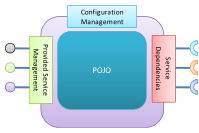
\includegraphics[width=0.5\textwidth]{contrib-astronef-ipojo}
    \caption{Un composant iPojo}\label{fig:contrib:astronef:ipojo}
\end{figure}
La figure~\ref{fig:contrib:astronef:ipojo} représente un composant dans l'implémentation \textit{iPojo}~\cite{Escoffier:ipojo}. Le code du composant (le \textit{POJO}, \textit{Plain Old Java Object}) est embarqué dans un conteneur auxquels sont accrochés des gestionnaires. Les trois couramment utilisés sont les gestionnaires de dépendances, de production de service, et de configuration. Ainsi, un composant peut s'exposer sur un registre, tout en dépendant d'autres services et en étant configurable.

\subsection{Les composants et services d'Astronef}
L'architecture d'Astronef est entièrement dirigé par les approches de composants orientés services. De multiples composants sont créés et instantiés, pour former une requête. Afin de pouvoir exécuter les requêtes, nous définissons trois services centraux :
\begin{itemize}
	\item[\textbf{Les services \textit{EventProcessor}}] ont deux primitives, l'une exécute une tâche, l'autre indique les \textit{EventProcessors} devant être exécutés avant soi-même.
	\item[\textbf{Le service \textit{Scheduler}}] permet la planification. Ses primitives permettent aux différents \textit{EventProcessor} d'exprimer leur volonté de s'exécuter. Ce service établit l'ordonnancement de ces demandes en fonction des contraintes des \textit{EventProcessor}s.
	\item[\textbf{Le service \textit{QueryRuntime}}] permet d'exécuter une requête. Il est lié à un \textit{Scheduler} et utilise la primitive \textit{next} de celui-ci pour connaître la prochaine tâche à exécuter.
\end{itemize}

Nous adoptons l'approche émise par~\cite{Carney:scheduling} en gérant l'ordonnancement par un service externes aux opérateurs, comme présenté dans la section~\ref{sec:rw:sgfd:infra}. Maintenant que nous avons vu les différents services nécessaire à l'exécution. Nous avons plusieurs types de composants que nous pouvons instantier par des services de fabriques :
\begin{itemize}
	\item[\textbf{Les flux ou relations} (entités)] : Fournissent les primitives nécessaires à leur manipulation par Astral. Ces entités servent de résultats intermédiaires (ou de tampons). De plus, ils permettent un service de notification. En cas de changement, les \textit{EventProcessor} abonnés sont notifiés. Ainsi, ces composants nécessitent un \textit{Scheduler} pour demander l'exécution de leurs abonnés.
	\item[\textbf{Les sources}] : Une source nécessite une entité qu'elle alimente grâce aux données issues d'origines diverses (protocoles réseaux, fichiers,...). Ce composant peut nécessiter le \textit{Scheduler} pour, entre autres, notifier sa fin de vie ce qui peut engendrer la fin de vie de la requête.
	\item[\textbf{Les opérateurs}] : Nécessitent $n$ entités en lecture, et une autre particulière en écriture. Ce composant doit fournir le service \textit{EventProcessor}. Les implémentations des opérateurs bloquants peuvent faire appel au \textit{Scheduler} pour planifier des exécutions ponctuelles.
	\item[\textbf{Les puits}] : Nécessitent une entité en lecture. Ce composant fournit le service \textit{EventProcessor} et doit être non-bloquant.
\end{itemize}

Ainsi pour créer une requête : l'utilisateur de l'intergiciel doit fournir un ou plusieurs composants sources et un composant puit. Par la suite, il demande à Astronef de lui instantier ses sources et son puit en configurant les composants selon sa volonté. Enfin, il spécifie l'expression algébrique liant les sources au puit.

\subsubsection{De l'importance de la réutilisation}
\textit{Astronef} permet une grande flexibilité grâce aux composants orientés services. Tout d'abord, chaque composant peut être configuré tout en gérant son cycle de vie, ce qui permet de réutiliser le même module pour plusieurs usages. Par exemple, supposons l'existence d'une source capable de récupérer une information périodiquement sur un dispositif $D$ via un protocole donné. Cette source peut être utilisée pour plusieurs requêtes sous différentes instances en ayant plusieurs configurations : différents dispositifs ou périodes d'acquisitions.

Cette abstraction sous forme de services permet surtout la substitution. En effet, nous pouvons remplacer tout composant par un autre supportant le même service. Nous utilisons ce principe pour sélectionner les meilleurs composants pour remplir le plus efficacement leurs rôles. De plus, l'utilisateur peut apporter ses propres implémentations pour étendre les capacités de l'intergiciel.

\section{Conclusion}
Après 20 années de recherche, la gestion de flux de données devient désormais suffisamment mature pour être appliqué massivement. Plusieurs produits commerciaux sont d'ailleurs maintenant utilisés en production. Toutefois, nous pouvons nous rendre compte que la complexité théorique de ces systèmes a été sous-estimé. De nombreux modèles ont été décrit pour représenter les flux de données et leurs traitements. Ces modèles sont encore remis en questions aujourd'hui au fur et à mesure des applications concrètes. 

Nous avons vu que le problème d'avoir une bonne connaissance du modèle et du comportement théorique des SGFD est crucial. En l'état, l'intégration des supports persistants reste ad-hoc et assisté par l'utilisateur. Un fonctionnement intégré avec une modélisation générique capable de gérer les deux modes d'interrogations de façon unifiée est donc indispensable pour manipuler correctement flux et relations persistantes. Similairement, les contributions sur l'optimisation de traitement des requêtes sont encore principalement ponctuelles. Afin d'appliquer un traitement efficace pour toute requête, il est nécessaire d'avoir une bonne connaissance théorique du traitement.

Notre contribution technique se concentrera sur trois points principaux :
\begin{itemize}
 \item[\textbf{Modélisation}] : Création d'Astral, algèbre de traitement des requêtes continues sur flux et relations temporelles. Nous accorderons de l'importance sur la prise en compte des problèmes relevés en section~\ref{sec:rw:sgfd:modeles:synthese}. Cette algèbre sera présenté dans le chapitre~\ref{chap:contrib:astral}
 \item[\textbf{Exécution}] : Mise en œuvre de l'intergiciel Astronef pour construire et exécuter efficacement une requête exprimée avec l'algèbre Astral. Ainsi, à partir d'une requête algébrique, il est possible de sélectionner le plan de requête qui semble le plus efficace grâce aux connaissances accumulés. Cette mise en œuvre sera développée dans le chapitre~\ref{chap:contrib:execution}.
 \item[\textbf{Persistance}] : Conception de l'extension Asteroid permettant l'intégration des requêtes continues sur flux et des requêtes sur support relationnel persistant. Ceci permettra de gérer la représentation du système observé ainsi que l'historisation des données dynamiques. Le support mathématique de cette intégration sera supporté par Astral et sa mise en œuvre par Astronef. Cette intégration sera effectuée dans le chapitre~\ref{chap:contrib:persistance}.
\end{itemize}

Grâce à ces contributions, il deviendra possible de mettre en œuvre un système d'observation générique applicable sur tout type de données. L'utilisateur devra exprimer des requêtes dans le langage algébrique Astral. Une fois ces requêtes écrites, nous serons garanti de leur mise en œuvre. Le tableau~\ref{tab:rw:contrib} résume l'ensemble des points d'analyses que nous nous étions fixés en section~\ref{sec:rw:supervision:criteres}.
\begin{table}[!ht]
\criteretabDonnee
    {Relationnel dérivé. Nous réutilisons les principes utilisés dans la gestion de flux et des bases de données.}
    {\good Modèle entité-relation augmenté pour supporter les flux.}
    {\good Requêtes sur tout type de données (flux, relations).}
\criteretabTraitement
    {\good Continue, Instantannée, Mixte}
    {\good Utilisation des requêtes continues des SGFD en tant qu'intégrateur.}
    {\meh Astral : langage de requête algébrique. Un langage purement déclaratif reste toutefois dérivable de ces fondations théoriques.}
    {\good Relationnel avec support \textbf{intégré} du dynamisme des données.}
\criteretabAdaptabilite
    {\good Spécification du modèle du système ainsi que des requêtes d'intégration (algébriques).}
    {\meh Pour l'analyse, la gestion de données multi-dimensionnelles des entrepôts utilisés est utilisé. Pour l'interrogation continue, utilisation d'un opérateur de préférences sur les flux.}
    {\good Infrastructure générique capable de supporter l'ajout d'opérateurs avec plusieurs implémentations.}
    {\good Héritage de l'efficacité des flux de données. Sélection du meilleur plan d'exécution pour chaque requête. Héritage des supports de grands volumes grâce aux entrepôts.}
\caption{Résumé de notre contribution selon nos critères}\label{tab:rw:contrib}
\end{table}

\begin{savequote}[6cm]
<< There's no need to go struttin' around and showin' off like that. 

\quad That's my job! >>
\qauthor{Rainbow Dash}
\end{savequote}

\chapter{Évaluation de performances}
\chaptertoc

Afin d'effectuer l'observation de systèmes, nous avons présenté dans les chapitres précédent un SGFD extensible capable de se coupler avec un SGBD. Pour permettre le déploiement de cette solution sur tout type de plateforme, nous devons nous assurer que notre système n'est pas trop lourd en terme de performance. Dans ce chapitre, nous analysons les capacités de notre système pour choisir le meilleur plan de requête en fonction de la requête \textit{Astral} que nous lui soumettons.

Tout d'abord, en section~\ref{sec:valid:perfs:cadre}, nous présentons notre cadre expérimental. Ensuite, en section~\ref{sec:valid:perfs:flux}, nous nous intéressons à l'optimisation de la gestion de flux de données en soit avec le support du \textit{benchmark} reconnu \textit{Linear Road}. Nous traitons l'efficacité du couplage avec le SGBD dans la section~\ref{sec:valid:perfs:flux}. Et enfin, nous présentons dans la section~\ref{sec:valid:perfs:prefs} comment nous pouvons ajouter des indications à Astronef pour exploiter au mieux les opérateurs de préférences que nous avons introduit dans le chapitre précédent.

\section{Cadre d'expérimentation}\label{sec:valid:perfs:cadre}
L'ensemble de la distribution Astronef-Asteroid est sous forme de \textit{bundles Java-OSGi}. Ainsi, ces prototypes peuvent être déployés sur toute plateforme possédant la technologie \textit{Java}. De plus, l'environnement \textit{OSGi} nous permet d'exploiter un environnement modulaire basé sur les architectures à service. La plateforme \textit{OSGi} doit embarquer le \textit{bundle} \textit{iPojo} (\url{http://felix.apache.org/site/apache-felix-ipojo.html}) pour pouvoir utiliser l'architecture à composants orientés service. Nous utilisons dans nos expériences la plateforme \textit{OSGi} \textit{Apache Felix} en version 3.0.2.

La distribution Astronef est fournie en trois \textit{bundles} obligatoires à déployer pour pouvoir utiliser l'ensemble des fonctionnalités présentés dans cette thèse (api core parser). Ces \textit{bundles} embarquent aussi le moteur \textit{Prova} (\url{http://prova.ws}, version 3.1.9 minimale) capable d'évaluer l'ensemble des règles présentées. Les extensions à Astronef sont aussi sous forme de \textit{bundles} dont les classes dépendent de l'\textit{api}. Astronef est disponible sous licence Apache 2.0 à l'adresse \url{http://astral.googlecode.com}.

Asteroid est une extension d'Astronef distribuée en un seul \textit{bundle}. Il embarque le SGBD \textit{H2} (\url{http://h2database.com}). Ce SGBD est entièrement en \textit{Java} ce qui permet une uniformité en terme de technologies. Le binaire ou le code source d'Asteroid n'est actuellement pas disponible au public.

L'ordinateur utilisé pour les expérimentations possède un processeur \textit{Intel Xeon}, quadricœur de fréquences 2.8Ghz. Il possède 6Go de mémoire vive et un disque dur d'une vitesse de 7200RPM. Le système d'exploitation installé est Linux Ubuntu 11.04. La plupart des expérimentations se sont faites dans un environnement clôt en isolant les processus sur trois cœurs dédiés afin d'éviter les interférences. Enfin, les expérimentations ont été faites dans des conditions les plus stables possible, après que le \textit{JIT} soit passé, après initialisation des caches internes et avec un \textit{garbage collector} (\textit{GC}) le plus stable possible.

Les performances sont mesurées par la latence d'un n-uplet. La latence est mesurée par la différence de timestamp système entre la source et le puits de la requête. Elle permet d'indiquer le temps total nécessaire au traitement d'un n-uplet. Le coût mémoire n'est pas compté, mais comme les trop grands coûts impactent le temps de traitement, notamment en \textit{Java} avec le \textit{GC}, nous supposons que cette métrique est représentative.
\section{Opérateurs de flux}
L'avantage de la gestion de flux est de pouvoir gérer la dynamique des données via des opérateurs dédiés. Astral est construite sur la sémantique a deux concepts, il nous faut donc définir les opérateurs flux vers relation (fenêtres) et relation vers flux (streamers). Puis, nous définirons et explorerons des opérateurs spécifiques à la gestion de flux étant : la gestion des modifications des relations et des \textit{batchs}.
\subsection{Fenêtres}
L'opérateur de fenêtre est un des opérateurs les plus étudiés dans la littérature. Toutefois, son comportement est encore flou sur certains points. La formalisation de son fonctionnement permettra donc une meilleure compréhension.
\subsubsection{Association position-\textit{batch}}
Avant de définir formellement l'opération de fenêtrage, nous avons besoin d'un outil pour gérer l'association entre la position d'un n-uplet et de son \textit{batch}. La fonction $\tau_S$ définit cette association. 
\begin{defi}[Fonction position-\textit{batch}]\label{def:tau}
    Soit $S$ un flux,

    La fonction $\tau_S : \N\cup\{-1\}\to \TN$ est la fonction associant un entier à l'identifiant de \textit{batch} du seul n-uplet présent à cette position.

    Par convention, $\tau_S(-1)=(t_0,0)$.
\end{defi}

Par corollaire de l'hypothèse fondamentale~\ref{hyp:ordres}, la fonction $\tau_S$ est donc croissante non-stricte. Ainsi, il est possible de définir une pseudo inverse $\rtau_S$ capable de donner une position (la maximale en l'occurence) pour un \textit{batch} donné.
\begin{coro}[Fonction pseudo-inverse $\tau$]
    Soit $S$ un flux,

    La pseudo-inverse $\rtau_S:\TN\to \N\cup\{-1\}$ existe et correspond à la plus grande position du \textit{batch} donné en entrée. Si aucun \textit{batch} n'existe, le plus proche est utilisé. Formellement, $$\forall b \in \TN, \qquad \tau_S^{-1}(b) = \sum_{n=-1}^{+\infty} n \indic_{[\tau_S(n),\tau_S(n+1)[}(b)$$
\end{coro}

De par sa nature, la fonction $\tau$ et sa pseudo-inverse partagent des propriétés intéressantes que nous pourrons réutiliser lors de démonstrations formelles.
\begin{prop}[Propriétés de $\tau$]
    Soit $S$ un flux, alors les propriétés suivantes sont correctes :
    \begin{eqnarray*}
        t_0 & \leq & \tau_S(0) \\
        \tau_S(\tau_S^{-1}(b)) & \leq & b \\
        n & \leq & \tau_S^{-1}(\tau_S(n))
    \end{eqnarray*}

    De plus, si $\exists s \in S$, $\BS(s)=b$, alors $\tau_S(\tau_S^{-1}(b)) = b$.
\end{prop}
\subsubsection{Description de séquences de fenêtres}
Afin de se rapproche le plus possible d'un aspect déclaratif, nous souhaitons décorréler l'opérateur de fenêtre en deux objets mathématiques : la description et l'opérateur exécutable. Ce dernier prendra une description en argument pour pouvoir représenter la relation temporelle résultante. Le principe des descriptions de séquences de fenêtres est assez simples, il suffit de décrire deux bornes évoluant de manière discrête, et un taux d'évaluation de ces bornes.

\begin{defi}[Description de Séquence de Fenêtre (DSF)]
    Soient $\D$ et $\D'$ pouvant être $\T$ ou $\N$, une description de séquence de fenêtre (DSF) est un triplet $(\alpha,\beta,r)$ tel que :
\begin{itemize}
    \item $r \in \D$ est le taux d'évaluation des bornes de la fenêtre
    \item $\alpha$ et $\beta$ sont deux fonction de $\N\to D'$ représentant l'évolution des bornes.
\end{itemize}

$\alpha(j)$ et $\alpha(j)$ définissent les $j\eme$ valeures des bornes. La première étant donnée pour $j=0$. Ces fonctions se doivent de vérifier les propriétés suivantes (en considérant $\D=\D'=\T$) :
$$\forall j \in \N, \begin{cases} \alpha(j) \leq \beta(j) & \textrm{le début est avant la fin}\\ \alpha(j) \geq t_0 & \textrm{le début existe} \\ \beta(j) \leq jr + \beta(0) & \textrm{la fin est accessible} \end{cases}$$
    Les conditions pour les autres cas pour $\D$ et $\D'$ sont évidentes par application des fonctions $\tau_S$ et $\tau_S^{-1}$.
\end{defi}

\begin{example}
    Nous souhaitons relever tous les $100$ relevés de charge processeur, les $10$ derniers relevés. Dans ce cas, nous souhaitons obtenir une séquence de fenêtres positionnelles générées tous les $100$ n-uplets ($r=100\in \N$). Nous appliquons des bornes positionnelles donc $\alpha,\beta \in (\N\to\N)^2$. La première fenêtre couvrira du $91\eme$ n-uplet au $100\eme$. Ainsi : $\alpha(0) = 91$ et $\beta(0) = 100$. L'évolution des bornes étant linéaire, nous avons donc :
\begin{eqnarray*}
 \alpha(j) &=& 100j+91\\
 \beta(j) &=& 100j + 100\\
 r & = & 100
\end{eqnarray*}
\end{example}

La création de fenêtre nécessite l'association entre les n-uplets du flux et le numéro de fenêtre décrit dans la \textit{DSF}. Pour cela, nous utilisons une \textit{fonction d'attente} utilisant les identifiants de \textit{batch}. Cette fonction donne le rang de la dernière fenêtre au moment indiqué par le batch. Le terme \textit{attente} est lié au fait que l'évaluateur devra attendre avant le prochain changement de $\gamma$.
Nous retrouvons dans cette fonction le caractère \textit{bloquant} des fenêtres.
\begin{defi}[Fonction d'attente $\gamma$]
    Soit $S$ un flux, soit $(\alpha,\beta,r)$ une DSF,

    La fonction d'attente de la DSF est une fonction $\TN \to \N$ associant un identifiant de \textit{batch} à l'identifiant de la dernière fenêtre complétée.
\begin{itemize}
 \item  Si $r\in\T$, cette fonction est définie par $\gamma : (t,i) \mapsto \left\lfloor \frac{t-\beta(0)}{r} \right\rfloor$.
 \item  Si $r\in\N$, cette fonction est définie par $\gamma : (t,i) \mapsto \left\lfloor \frac{\rtau_S(t,i)-\beta(0)}{r} \right\rfloor$.
\end{itemize}
\end{defi}
\begin{example}
    En reprenant l'exemple précédent, après simplification nous obtenons : $$\gamma(b) = \left\lfloor \frac{\rtau_S(b)}{100}\right\rfloor-1.$$
    Si nous supposons que le flux produit un n-uplet par seconde (ainsi, $\rtau_S(t,i) = \lfloor t/1s \rfloor$) : alors $\gamma(1024s,0) = \left\lfloor \frac{1024}{100}\right\rfloor-1 = 9$. Nous avons donc bien la $10\eme$ fenêtre ($j=9$) comme la dernière fenêtre créée à ce moment.
\end{example}

\subsubsection{L'opérateur}
Il devient désormais possible de définir un opérateur permettant  de générer une relation temporelle à partir d'un flux donné. Cette relation temporelle gère ses changements d'état grâce à la fonction $\gamma$. De manière générale, une DSF peut être ramenée simplement à une expression plus générale $(\alpha,\beta,\gamma)$ ce que nous utiliserons pour la définition de séquence de fenêtres.
\begin{defi}[Opérateur de Séquence de Fenêtres]
	Soit $S$ un flux et $(\alpha, \beta, \gamma)$ une description de séquence,
	
	L'opérateur de séquence de fenêtres est défini par : $\forall b \in \TN$, 
	\begin{itemize}
		\item Si $\gamma(b) \geq 0$, 
		\begin{itemize}
			\item Si la description possède des bornes temporelles :
			$$S[\alpha,\beta,\gamma](b) = \left\{s\in S, \ (\alpha(\gamma(b)),0)\leq \BS(s) \leq (\beta(\gamma(b)),i)\right\}$$
			\item Si la description possède des bornes positions :
			$$E(b) = \left\{s\in S, \ \tau_S(\alpha(\gamma(b)))\leq \BS(s) \leq \tau_S(\beta(\gamma(b)))\right\}$$
			$$S[\alpha,\beta,\gamma](b) = \{s \in E(b) / (\#E(b) - \pos_{E(b)}(s)) \leq \beta(\gamma(b)) - \alpha(\gamma(b))$$
		\end{itemize}
		\item Si $\gamma(b) <0$ alors $S[\alpha,\beta,\gamma](b) = \emptyset$
	\end{itemize}
\end{defi}

Plusieurs remarques peuvent être formulées sur cette définition. Tout d'abord, les expressions sont différentes si les bornes sont positionnelles ou temporelles. Pour les fenêtres temporelles, l'opérateur inclue les n-uplets dont l'identifiant de \textit{batch} s'étend :
\begin{itemize}
	\item[\textbf{depuis}] le premier \textit{batch} de la fenêtre : $(\alpha(\gamma(t,i)),0)$, i.e. ceux dont le \textit{timestamp} est supérieur à la borne inférieur.
	\item[\textbf{jusqu'au}] dernier \textit{batch} de la fenêtre : $(\beta(\gamma(t,i)),i)$. Ce qui correspond au $i\eme$ \textit{batch} ayant le \textit{timestamp} inférieur ou égal à la borne.
\end{itemize}
Il est important de voir que $S[\alpha,\beta,\gamma]$ pourra changer à l'arrivée d'un nouveau \textit{batch}, même si le \textit{timestamp} ne change pas. Ne pas inclure ces modifications ferait perdre des données de dynamicités à la fenêtre. Nous retrouvons donc les problématiques explorées dans la section~\ref{sec:rw:sgfd:modeles}.

Pour les fenêtres positionnelles, la gestion est plus délicate. Si nous considérons que le flux réparti ses \textit{batchs} (donc un n-uplet par \textit{batch}), alors $E(b) = S[\alpha,\beta,\gamma](b)$. Mais dans le cadre général, $E(b)$ contient l'ensemble des n-uplets potentiels et la séquence $S[\alpha,\beta,\gamma](b)$ en est un sous-ensemble dont la taille est exactement celle décrite dans la DSF (sélections des n-uplets les plus récents). De plus, nous remarquons que $\gamma$ en positionnel est dirigé par $\rtau_S$ qui fournit la position maximale en cas d'égalité de \textit{batch}, ce qui nous garanti de couvrir l'ensemble des n-uplets concernés.

	
\begin{example}
	La figure~\ref{fig:contrib:astral:fenetres} montre l'évolution d'une séquence où la fenêtre glisse de $2$ secondes toutes les $2$ secondes ($r=2$) avec une taille constante de $3$ secondes. $t_0 = 0$ par simplicité ici. 
La première fenêtre possède les bornes $\alpha(0) = t_0+ 0s$ et $\beta(0) =t_0+3s$. Le glissement étant de $2s$ la description de fenêtre est donc $$\forall j \in \N, \begin{cases} \alpha(j)  & =\ i*2s+t_0 \\ \beta(j) & = \ j*2s+3s+t_0\end{cases}$$
La relation temporelle généré par cette DSF peut être noté $S[2js,2js+3s,2s]$.  Le calcul de son état à un instant est simple. Prenons le batch $(t_0+5.5s,0)$. La fenêtre a calculer est la fenêtre numérotée $\gamma(t_0+5.5s,0) = \left\lfloor \frac{t_0+5.5s-\beta(0)}{r}\right\rfloor = 1$. Ainsi : $S[2js,2js+3s,2s](t_0+5.5s,0) = F_1 = \{s_4,s_5,s_6,s_7,s_8\}$.
\end{example}
\begin{figure}[ht]
	\centering
	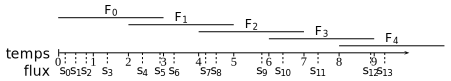
\includegraphics[width=0.7\textwidth]{contrib-astral-fenetres}
	\caption{Séquence de fenêtre de taille $3s$ glissante de $2s$}\label{fig:contrib:astral:fenetres}
\end{figure}

\subsubsection{Fenêtres partitionnées}
L'opérateur de fenêtres partitionnée est très utilisé pour appliquer la même séquences de fenêtres à des sous-flux. Les opérateurs partitionnés sont tous décrit de la même manière. Le principe, illustré dans la figure~\ref{fig:contrib:astral:partition} est de divisé le flux suivant un (ou des) attributs $A$ donné. Sur chacun de ces sous-flux est appliqué un opérateur quelconque. Par la suite, une union est appliquée.
\begin{figure}[ht]
	\centering
	\includegraphics[width=0.9\textwidth]{contrib-astral-partition}
	\caption{Principe d'un opérateur partitionné}\label{fig:contrib:astral:partition}
\end{figure}
\begin{defi}[Séquence de fenêtre partitionnée]
	Soient $S$ un flux, $a_1,...,a_k$ un ensemble d'attributs du schéma de $S$, et $(\alpha,\beta,\gamma)$ une DSF,
	
	Soit $\cup^*$ l'union relationnelle conservatrice des identifiants physiques, 

	Alors la séquence de fenêtre $(\alpha,\beta,\gamma)$ partitionnée par $a_1,...,a_k$ est définie par :
	$$S[a_1...a_k/\alpha,\beta,\gamma] = \mathop{\bigcup\null^*}_{a\in Dom(a_1,...,a_k)} (\sigma_{(a_1,...,a_k)=a} S)[\alpha,\beta,\gamma]$$
\end{defi}

Nous remarquons que nous utilisons la définition conservatrice de l'union relationnelle présenté dans la section précédente, ainsi l'ordre naturel décrit dans le flux d'entrée pourra être retrouvé dans la relation de sortie.
\begin{example}
	L'exemple le plus courant étant la représentation de l'état actuel d'un système à partir d'un flux. Supposons un flux d'entrée $DeviceCPU(deviceId,cpu,\t)$, nous donnant les relevés de charge de processeur. Soit la description de fenêtre rapportant le dernier n-uplet d'un flux : $(1j,1j,1)$. Nous pouvons obtenir la relation temporelle représentant pour chaque dispositif $deviceId$, la dernière valeure connue de $cpu$ et son \textit{timestamp de mesure} $\tau$ : $$DeviceCPU[id/1j,1j,1]$$

	Cet exemple illustre comment nous pouvons passer d'un flux brut à une représentation (dynamique) d'un \textbf{contexte}.
\end{example}

Par la suite, nous utiliserons plusieurs notations simplifiés pour désigner des descriptions de fenêtres courantes décrites dans le tableau~\ref{tab:windows}.
\begin{table}
\centering
\begin{tabular}{c||p{0.4\textwidth}|p{0.4\textwidth}}
  & Définition & Équivalence \\ \bottomrule
 $[L]$ & $[j,j,1]$ &  \\ 
 & \multicolumn{2}{p{0.8\textwidth}}{La séquence de fenêtre où chaque fenêtre ne contient que le dernier n-uplet du flux. Cette séquence est égale à $[B]$ si le flux réparti ses n-uplets avec un n-uplet par \textit{batch}.} \\ \hline
 $[B]$ & $[\tau_S^{-1}(\tau_S(j)^-)+1,j,1]$ & $\{s\in S, \BS(s) = \tau_S\circ\tau_S^{-1}(b)\}$ \\ 
 & \multicolumn{2}{p{0.8\textwidth}}{Séquence de fenêtre où chaque fenêtre contenient le dernier \textit{batch}.} \\\hline
 $[\infty]$ & $[0,j,1]$ & $\{s\in S, \BS(s) \leq b\}$ \\
 & \multicolumn{2}{p{0.8\textwidth}}{Séquence accumulative contenant tout le flux jusqu'au \textit{batch} courant.} \\\hline
 $[T\ r]$ & $[\max(rj-r+t_0,t_0),rj+t_0,r]$ &  \\
 & \multicolumn{2}{p{0.8\textwidth}}{Fenêtre temporelle de taille $r$ se déplaçant toutes les $r$ unités de temps.} \\\hline
 $[P\ r]$ & $[\max(rj-r,0),rj,r]$ &  \\
 & \multicolumn{2}{p{0.8\textwidth}}{Fenêtre positionnelle de taille $r$ n-uplets se déplaçant tous les $r$ n-uplets.} \\
 \toprule
\end{tabular}
\caption{Liste des fenêtres courantes} \label{tab:windows}
\end{table}

Il est important de noter que les équivalences citées sont toutefois non triviales, des démonstrations formelles sont fournies en annexes.

\subsection{Streamers}
\subsection{Domaine}
\subsection{Spread}
\section{Choix du plan de jointure dans Asteroid}\label{sec:valid:perfs:couplage}
En section~\ref{sec:contrib:asteroid:reecriture:join}, nous avons présenté un opérateur capable de faire une jointure $\ssjoin$ entre une relation temporelle d'Astronef et une relation issue d'un SGBD. Deux plans ont été présenté : le plan \textbf{P1} applique la jointure dans Astronef en utilisant la relation temporelle issue du SGBD comme cache local ; le plan \textit{P2} quant à lui exécute l'opération de jointure à l'intérieur du SGBD pour exploiter ses capacités. Alors que l'optimisation poussant les opérateurs au plus proche du SGBD semble efficace dans la plupart des cas, nous voyons dans cette section que ce n'est pas toujours le cas pour cette opération.

\subsection{Jointure sur une relation statique}
Nous exécutons ici la requête $CPUMem$ présenté en section~\ref{sec:valid:domvision:requetes:historisation}. Pour rappel, cette requête implique une jointure avec $Application \Join Monitorable$ pour pouvoir identifier le flux de métriques processeurs et mémoires. Voici les paramètres d'expérimentations que nous fixons :
\begin{itemize}
	\item Les relations temporelles \textit{Monitorable} et \textit{Applications} sont considérées statiques
	\item La cardinalité d'\textit{Applications} est $N$
	\item La cardinalité de \textit{Devices} est $0.2N$ et celle de \textit{Monitorable} est de $1.2N$
	\item Il existe un index \textit{Application(monitorableId)}, \textit{Monitorable(monitorableId)} et sur \textit{Monitorable(name)}
	\item Il y a toujours suffisamment de mémoire pour exécuter les requêtes \textit{SQL}.
\end{itemize}

La requête \textit{SQL} automatiquement généré et donnée aux composants \textit{dbjoin} et \textit{dbsource} est la suivante :
\begin{lstlisting}[language=SQL]
SELECT deviceId as monitorableId, name 
FROM Application NATURAL JOIN Monitorable
\end{lstlisting}

\begin{figure}[ht]
	\centering
	\includegraphics[width=0.66\textwidth]{valid-perfs-asteroid-static}
	\caption{Performance d'une jointure sur catalogue statique}\label{fig:valid:perfs:asteroid:static}
\end{figure}

\textbf{Résultats} : La figure~\ref{fig:valid:perfs:asteroid:static} montre la latence des deux plans de requête \textbf{P1} et \textbf{P2}. Les expérimentations ont montré que le plan \textit{P1} est meilleur et plus stable sur $N$. Bien entendu, cela ne pourra pas être le cas pour des valeurs très larges de $N$. Dans notre cadre expérimental, le \textit{hash-join} ne semble pas être le facteur limitant à $100\mu s$, car cela consiste à interroger une table de hachage constituée une seule fois. Le coût du \textit{scheduling} et d'autres tâches de l'intergiciel deviennent des facteurs limitants. 

Le plan \textbf{P2} est plus coûteux car pour chaque n-uplet, le composant doit se connecter au SGBD et exécuter la requête. Bien que la requête soit préparé, cela introduit un coût supplémentaire. Ce plan utilise l'index stocké sur disque dur, mais ses performances sont moindre comparé à un accès direct à une table de hachage en mémoire.

Si les relations \textit{Monitorable} ou \textit{Applications} sont mis à jour, cela introduit un surcout pour recalculer la table de hachage. Toutefois, le coût est absorbé au fur et à mesure du temps si les relations sont mises à jour rarement. Ainsi, le choix de \textbf{P1} est le meilleur pour la jointure avec des relations stables.

\subsection{Jointure sur un agrégat historique}
Dans cette seconde expérimentation, nous exécutons la requête $HistAvgCPU$ vu dans la section~\ref{sec:valid:domvision:requetes:alerte}. Pour rappel, cette requête joint une relation temporelle avec un agrégat effectué sur historique. Voici les paramètres de notre expérience :
\begin{itemize}
	\item L'historique est mise à jour dès que possible par un processus de collecte extérieur ($CPUMem$ par exemple).
	\item Il existe $D$ identifiants d'équipement et $M$ valeurs historique par identifiants.
	\item Il y a un index sur \textit{HistCPU(monitorableId)}.
\end{itemize}

La requête \textit{SQL} générée et donnée en paramètre à \textit{dbjoin} et \textit{dbsource} est la suivante : 
\begin{lstlisting}
SELECT monitorableId, AVG(cpu) as avg FROM HistCPU GROUP BY monitorableId
\end{lstlisting}

\begin{figure}[ht]
\subfigure[Performance globale]{\includegraphics[width=0.48\linewidth]{valid-perfs-asteroid-aggregate}\label{fig:valid:perfs:asteroid:aggregate}}
\subfigure[Performance de l'agrégat avec sélection sur identifiant]{\includegraphics[width=0.48\linewidth]{valid-perfs-asteroid-aggregate-select}\label{fig:valid:perfs:asteroid:aggregate:select}}
\caption{Performance de la jointure avec agrégat en utilisant la sélection ou non}\label{fig:valid:perfs:asteroid:agg}
\end{figure}

\textbf{Résultats} : Dans cette expérience, nous avons pu remarquer que les performances de la requête \textit{SQL} de \textit{dbsource} ne dépend que de la taille de l'historique $(M.D)$. Toutefois, ce n'est pas le cas pour un agrégat utilisant une sélection sur l'identifiant avec \textit{dbjoin}, qui ne dépend principalement que de $M$. La figure~\ref{fig:valid:perfs:asteroid:aggregate} représente l'évolution de la latence de la requête d'agrégat avec et sans la sélection\footnote{La perte de performance massive observée après $4M$ de n-uplets est due au \textit{buffering} qui ne peut être fait en mémoire et le disque est utilisé. Ce fait a été confirmé par les développeurs d'\textit{H2}.}. La figure~\ref{fig:valid:perfs:asteroid:aggregate:select} représente l'évolution de la latence en variant $M$ pour l'agrégat avec sélection.

La performance dépend des caractéristiques de l'historique. Plus nous avons un $M$ petit, plus nous avons une petite latence pour le plan \textbf{P2}. La latence de \textbf{P2} est bornée entre les deux courbes de la figure~\ref{fig:valid:perfs:asteroid:aggregate} comme le cas $M=10$ représente le minimum de latence et $D=1$ (équivalent à aucune sélection) est le pire cas. Le choix du plan est clairement en faveur du plan \textbf{P2} car son pire cas a des performances similaires à \textbf{P1}. Dans l'expérience précédente, nous avions supposé pouvoir absorbé le coût de mise à jour. Ce n'est pas le cas ici car l'historique est régulièrement mis à jour.

\subsubsection{D'autres stratégies}
Si le résultat de la requête peut être dégradé, il est possible d'utiliser \textit{dbsource} est mode périodique. Dans ce cas, nous pouvons évaluer la condition limite pour passer d'un plan à l'autre en regardant les coûts mesurés dans la figure~\ref{fig:valid:perfs:asteroid:agg}.

Nous pouvons toutefois trouver une autre réécriture exacte. Lorsque la requête est déployé, il est possible de faire une distinction entre le passé $(CPUMemHistory^{t_0})$ et le futur représenté par le flux $CPUMem$. En supposant que l'agrégat est séparable par les moyens décrit dans la section~\ref{sec:rw:sgfd:optim:fenetres}, alors nous pouvons séparer les calculs sur le passé et le futur. L'agrégat passé est un calcul instantané effectué par \textit{dbsource} est mode \textit{one-shot}. L'agrégat futur est calculé par les opérateurs $_{id}\G[\infty]$. Or, ces opérateurs peuvent être regroupés en un seul macro-bloc capable de calculer l'agrégat avec un coût mémoire borné.
\section{L'avantage du mode incrémental dans Best/KBest}\label{sec:valid:perfs:prefs}
\subsection{Les algorithmes des opérateurs}
\subsection{Le jeu de données}
\subsection{Résultats}

\section{Conclusion}
Après 20 années de recherche, la gestion de flux de données devient désormais suffisamment mature pour être appliqué massivement. Plusieurs produits commerciaux sont d'ailleurs maintenant utilisés en production. Toutefois, nous pouvons nous rendre compte que la complexité théorique de ces systèmes a été sous-estimé. De nombreux modèles ont été décrit pour représenter les flux de données et leurs traitements. Ces modèles sont encore remis en questions aujourd'hui au fur et à mesure des applications concrètes. 

Nous avons vu que le problème d'avoir une bonne connaissance du modèle et du comportement théorique des SGFD est crucial. En l'état, l'intégration des supports persistants reste ad-hoc et assisté par l'utilisateur. Un fonctionnement intégré avec une modélisation générique capable de gérer les deux modes d'interrogations de façon unifiée est donc indispensable pour manipuler correctement flux et relations persistantes. Similairement, les contributions sur l'optimisation de traitement des requêtes sont encore principalement ponctuelles. Afin d'appliquer un traitement efficace pour toute requête, il est nécessaire d'avoir une bonne connaissance théorique du traitement.

Notre contribution technique se concentrera sur trois points principaux :
\begin{itemize}
 \item[\textbf{Modélisation}] : Création d'Astral, algèbre de traitement des requêtes continues sur flux et relations temporelles. Nous accorderons de l'importance sur la prise en compte des problèmes relevés en section~\ref{sec:rw:sgfd:modeles:synthese}. Cette algèbre sera présenté dans le chapitre~\ref{chap:contrib:astral}
 \item[\textbf{Exécution}] : Mise en œuvre de l'intergiciel Astronef pour construire et exécuter efficacement une requête exprimée avec l'algèbre Astral. Ainsi, à partir d'une requête algébrique, il est possible de sélectionner le plan de requête qui semble le plus efficace grâce aux connaissances accumulés. Cette mise en œuvre sera développée dans le chapitre~\ref{chap:contrib:execution}.
 \item[\textbf{Persistance}] : Conception de l'extension Asteroid permettant l'intégration des requêtes continues sur flux et des requêtes sur support relationnel persistant. Ceci permettra de gérer la représentation du système observé ainsi que l'historisation des données dynamiques. Le support mathématique de cette intégration sera supporté par Astral et sa mise en œuvre par Astronef. Cette intégration sera effectuée dans le chapitre~\ref{chap:contrib:persistance}.
\end{itemize}

Grâce à ces contributions, il deviendra possible de mettre en œuvre un système d'observation générique applicable sur tout type de données. L'utilisateur devra exprimer des requêtes dans le langage algébrique Astral. Une fois ces requêtes écrites, nous serons garanti de leur mise en œuvre. Le tableau~\ref{tab:rw:contrib} résume l'ensemble des points d'analyses que nous nous étions fixés en section~\ref{sec:rw:supervision:criteres}.
\begin{table}[!ht]
\criteretabDonnee
    {Relationnel dérivé. Nous réutilisons les principes utilisés dans la gestion de flux et des bases de données.}
    {\good Modèle entité-relation augmenté pour supporter les flux.}
    {\good Requêtes sur tout type de données (flux, relations).}
\criteretabTraitement
    {\good Continue, Instantannée, Mixte}
    {\good Utilisation des requêtes continues des SGFD en tant qu'intégrateur.}
    {\meh Astral : langage de requête algébrique. Un langage purement déclaratif reste toutefois dérivable de ces fondations théoriques.}
    {\good Relationnel avec support \textbf{intégré} du dynamisme des données.}
\criteretabAdaptabilite
    {\good Spécification du modèle du système ainsi que des requêtes d'intégration (algébriques).}
    {\meh Pour l'analyse, la gestion de données multi-dimensionnelles des entrepôts utilisés est utilisé. Pour l'interrogation continue, utilisation d'un opérateur de préférences sur les flux.}
    {\good Infrastructure générique capable de supporter l'ajout d'opérateurs avec plusieurs implémentations.}
    {\good Héritage de l'efficacité des flux de données. Sélection du meilleur plan d'exécution pour chaque requête. Héritage des supports de grands volumes grâce aux entrepôts.}
\caption{Résumé de notre contribution selon nos critères}\label{tab:rw:contrib}
\end{table}

